\chapter{The p-Block I: Boron, Carbon and Nitrogen Groups}\label{ch:b1:p-block-13-15}

The air we breathe is four-fifths nitrogen, yet plants starve for it: the
\ce{N#N} triple bond is so strong that almost nothing breaks it. For most
of history, the nitrogen of crops came from manure, from bacteria living
on the roots of legumes, and from mined nitrates. Early in the twentieth
century a reaction between nitrogen and hydrogen over an iron \omterm{def:b1:elementary-steps:catalyst}{catalyst}
changed that; today the world makes about 160 million tonnes of nitrogen
a year as ammonia, and roughly half the nitrogen in a human body has
passed through an ammonia plant. \omterm{def:b1:periodicity:table}{Groups} 13, 14 and 15 hold the elements of
that story --- nitrogen and phosphorus for fertilisers, carbon and
silicon for life and rocks, boron and aluminium for glass and light
alloys. This chapter surveys them with the tools of the earlier chapters.

\begin{recall}
\omterm{def:b1:crystals-metals:allotropy}{Allotropes} of carbon and the structure of silicon and silica
(\cref{ch:b1:crystals-ionic-covalent}); the character of oxides
(\cref{def:b1:s-block:oxide-character}); \omterm{def:b1:nernst:oxidation-number}{oxidation numbers} and \omterm{def:b1:nernst:electrode-potential}{standard
potentials} (\cref{ch:b1:nernst}); \omterm{def:b1:precipitation:amphoteric-hydroxide}{amphoteric hydroxides}
(\cref{ch:b1:precipitation}); equilibrium constants from Gibbs energies
(\cref{ch:b1:extent-q-and-k}).
\end{recall}
% ledger: usgs:N-world-2025

\begin{omfigure}
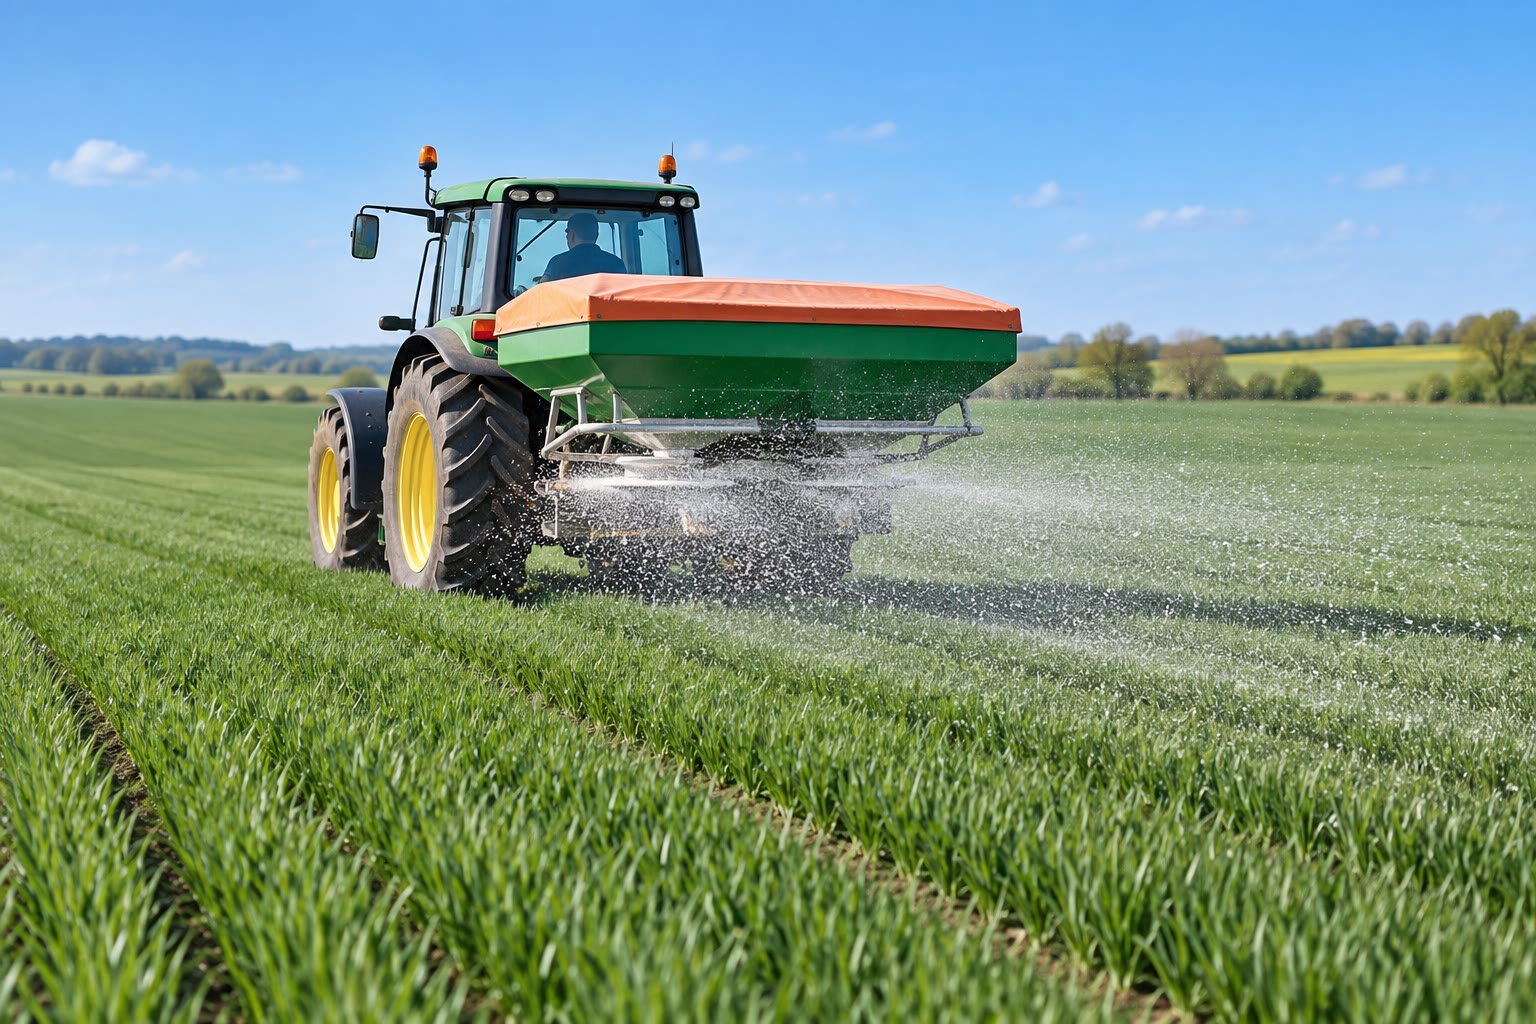
\includegraphics[width=0.55\linewidth]{images/book2/ai/b1-27-fertiliser-field.jpg}

{\small Spreading a nitrogen fertiliser on a wheat field. Most of it was
made from the nitrogen of the air by the Haber--Bosch process.}
\end{omfigure}

\section{Group 13: boron and aluminium}

Boron is a \omterm{def:b1:periodicity:metalloid}{metalloid} that forms covalent compounds with an incomplete
octet: in \ce{BF3} and boric acid \ce{B(OH)3}, boron has six \omterm{def:b1:quantum-numbers:configuration}{valence
electrons} and acts as a \omterm{def:b1:lewis-resonance-vsepr:lewis-acid}{Lewis acid} (\cref{ch:b1:lewis-resonance-vsepr}).
Boric acid is a \omterm{def:b1:predominant-reaction:strong-acid}{weak acid} not by losing a proton but by accepting a
hydroxide ion, \ce{B(OH)3 + 2H2O <=> B(OH)4- + H3O+}. Borax, a sodium
borate, is used in glass and detergents.

\begin{definition}[Oxoacid]\label{def:b1:p-block-13-15:oxoacid}
An \emph{oxoacid}\index{oxoacid} is an acid in which the acidic hydrogen
atoms are bound to oxygen atoms that are bound to a \omterm{def:b1:complexation:complex}{central atom}:
\ce{B(OH)3}, \ce{H2CO3}, \ce{HNO3} (\ce{HO-NO2}), \ce{H3PO4}
(\ce{(HO)3PO}), \ce{H2SO4}. The more oxygen atoms without hydrogen around
the \omterm{def:b1:complexation:complex}{central atom}, the stronger the acid.
\end{definition}

Aluminium, below boron, is a metal, but its small, highly charged ion
gives it an \omterm{def:b1:s-block:oxide-character}{amphoteric oxide} and hydroxide (\cref{sec:b1:precipitation:amphoteric}).
Its ore is bauxite, a mixture of aluminium hydroxides with iron oxides and
silica; in 2025 the world mined about 440 million tonnes of bauxite and
refined about 150 million tonnes of alumina from it.
% ledger: usgs:bauxite-world-2025, usgs:alumina-world-2025

\begin{proposition}[The Bayer process]\label{prop:b1:p-block-13-15:bayer}
Hot concentrated sodium hydroxide dissolves the aluminium of bauxite as
\ce{Al(OH)4-} and leaves the iron oxides (red mud); cooling and seeding the
filtered solution precipitates pure \ce{Al(OH)3}, calcined to alumina,
\ce{2Al(OH)3 -> Al2O3 + 3H2O}.
\end{proposition}

\begin{proof}
\ce{Al(OH)3(s) + OH- <=> Al(OH)4-} has $K = 10^{-1.23}$ at
\qty{25}{\celsius} (\cref{ch:b1:precipitation}): at high \ce{[OH-]} the
aluminium is in solution, while iron(III) hydroxide, not amphoteric,
stays solid (\cref{exo:b1:precipitation:12}). Dilution and cooling lower
the \ce{[OH-]} and shift the quotient so that $Q > K$ for the reverse
reaction: the hydroxide precipitates. Calcination removes water.
\end{proof}

Alumina is then reduced to aluminium by electrolysis in molten cryolite,
an industry studied in the Year~2 volume.

\begin{omfigure}
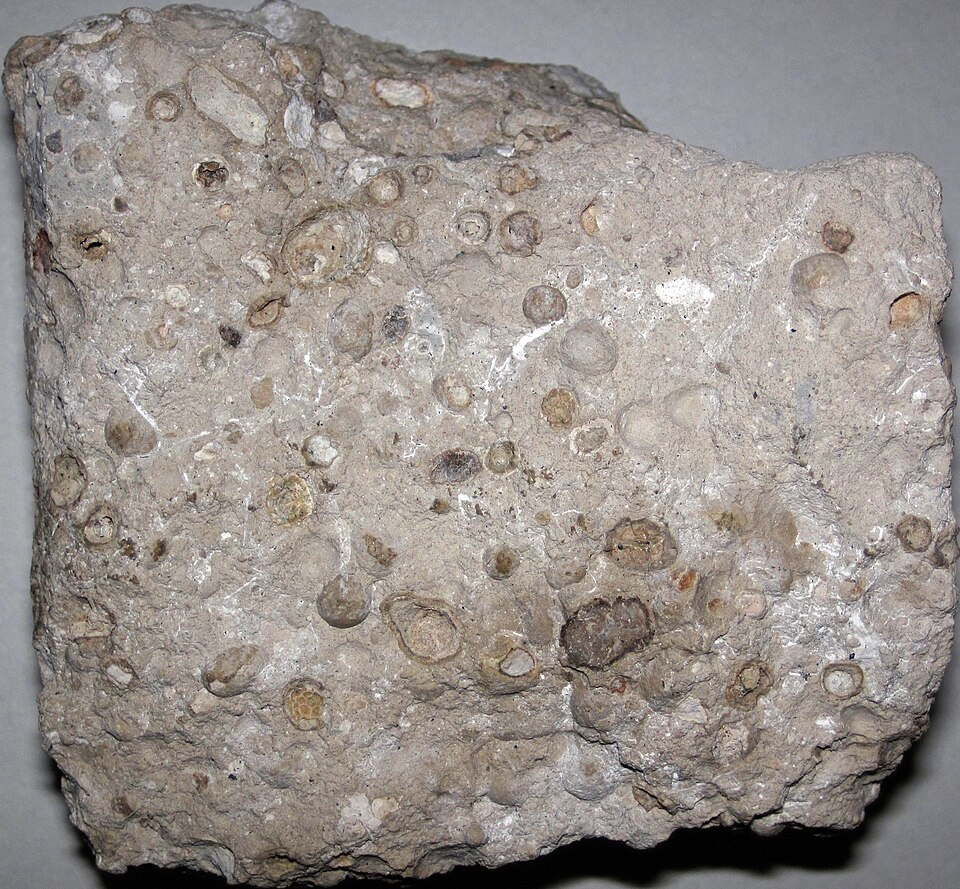
\includegraphics[height=3.6cm]{images/book2/bauxite.jpg}\hspace{0.4em}%
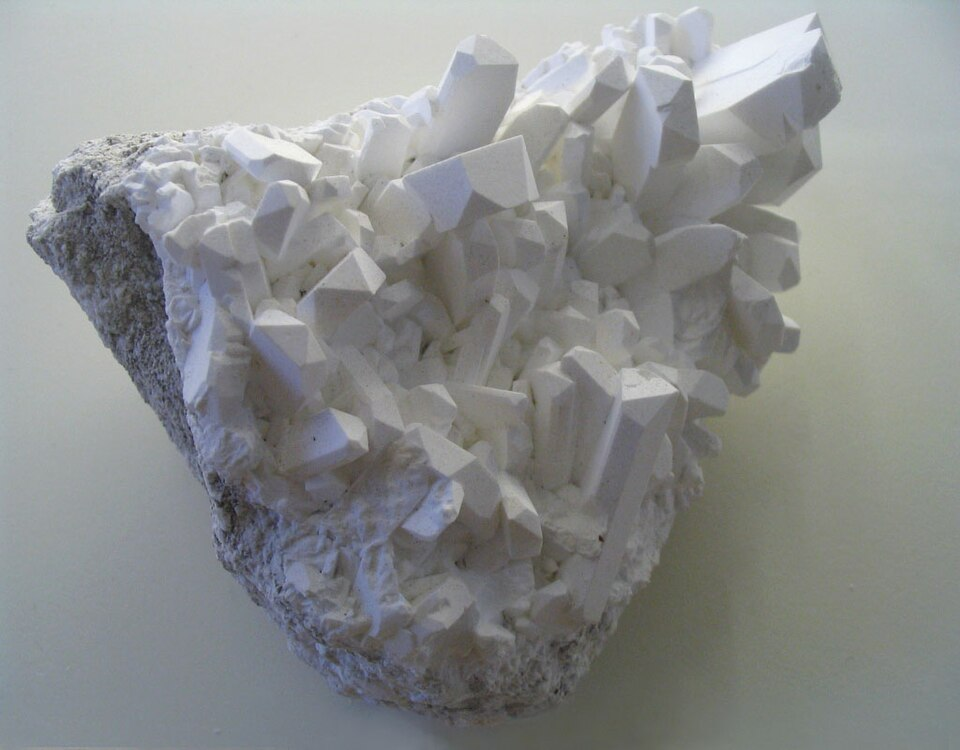
\includegraphics[height=3.6cm]{images/book2/borax.jpg}\hspace{0.4em}%
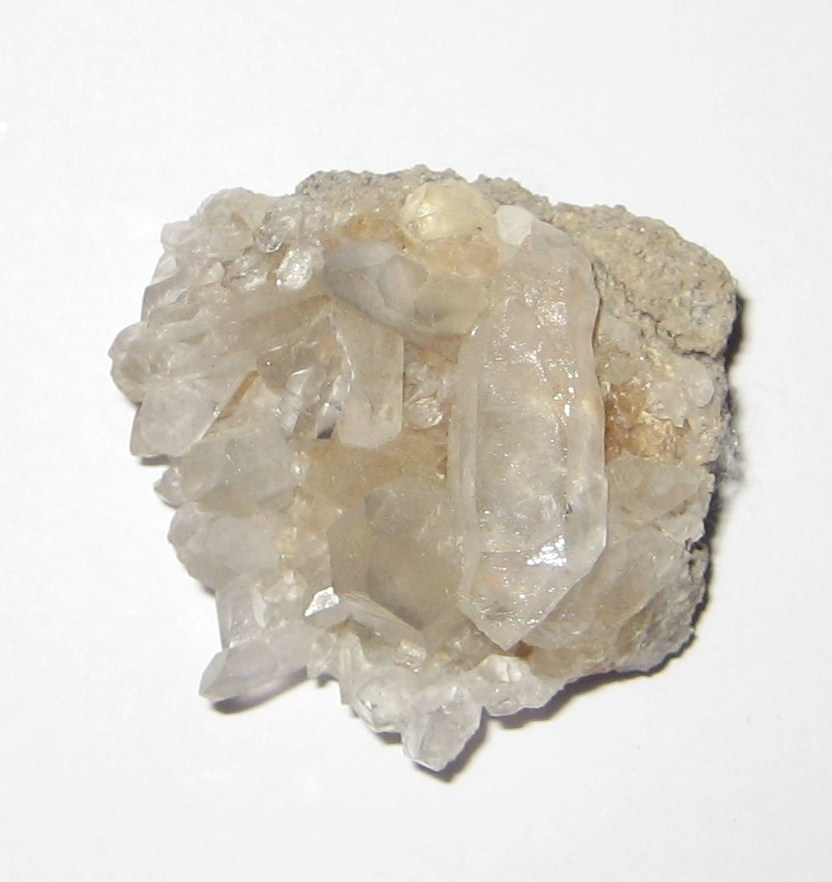
\includegraphics[height=3.6cm]{images/book2/quartz.jpg}\hspace{0.4em}%
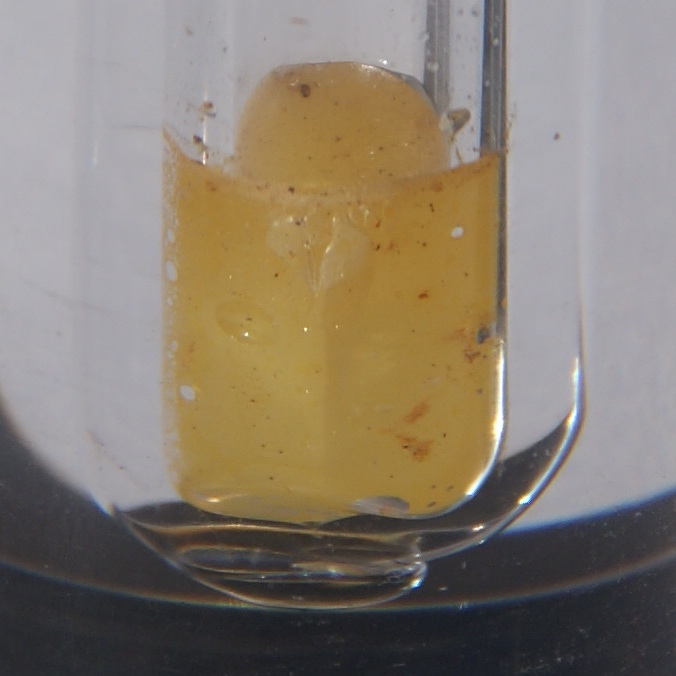
\includegraphics[height=3.6cm]{images/book2/white-phosphorus.jpg}

{\small From left to right: pisolitic bauxite (James St. John, CC BY 2.0);
borax \omterm{def:b1:crystals-metals:crystal}{crystals} (Aram Dulyan, public domain); a cluster of quartz \omterm{def:b1:crystals-metals:crystal}{crystals},
\ce{SiO2} (Stephanie Clifford, CC BY 2.0); white phosphorus, with a little
red phosphorus, kept under water because it ignites in air (Hi-Res Images
of Chemical Elements, CC BY 3.0). All Wikimedia Commons.}
\end{omfigure}

\section{Group 14: carbon and silicon}

Carbon and silicon both form four bonds, but differently. Carbon forms
strong double bonds: \ce{CO2} is a molecule, \ce{O=C=O}, a gas. Silicon
hardly does: \ce{SiO2} is a covalent network of \ce{SiO4} tetrahedra
sharing all their corners, a hard solid, quartz (\cref{ch:b1:crystals-ionic-covalent}).
Carbon dioxide is an \omterm{def:b1:s-block:oxide-character}{acidic oxide}, giving carbonic acid, hydrogencarbonates
and carbonates (\cref{ch:b1:predominant-reaction}); silica is an \omterm{def:b1:s-block:oxide-character}{acidic
oxide} too, attacked by molten alkali to give silicates.

\begin{proposition}[Silicate units]\label{prop:b1:p-block-13-15:silicate-units}
Silicates are built of \ce{SiO4} tetrahedra; the number of corners shared
with other tetrahedra fixes the formula of the anion: none, \ce{SiO4^4-}
(isolated tetrahedra); two, chains $(\ce{SiO3})_n^{2n-}$; three, sheets
$(\ce{Si2O5})_n^{2n-}$; four, the neutral framework \ce{SiO2}.
\end{proposition}

\begin{proof}
A shared oxygen belongs half to each tetrahedron. A tetrahedron sharing
$k$ corners owns $4 - k$ oxygen atoms entirely and $k$ by halves: $4 -
k/2$ oxygens per silicon. Each unshared oxygen carries a charge $-1$ (it
has one bond), each shared one none: the charge per silicon is
$-(4 - k)$. $k = 0$: \ce{SiO4^4-}; $k = 2$: \ce{SiO3^2-} per silicon;
$k = 3$: \ce{SiO_{2.5}^-}, that is \ce{Si2O5^2-}; $k = 4$: \ce{SiO2}.
\end{proof}

\begin{omfigure}
\begin{tikzpicture}[font=\small, line join=round]
  % one SiO4 tetrahedron in perspective
  \begin{scope}
    \coordinate (t) at (0,1.2); \coordinate (a) at (-1.0,-0.5);
    \coordinate (b) at (1.0,-0.5); \coordinate (c) at (0.25,0.05);
    \draw[thick, omDef] (t) -- (a) -- (b) -- cycle; \draw[thick, omDef] (t) -- (b);
    \draw[dashed, omDef] (a) -- (c) -- (b) (t) -- (c);
    \foreach \p in {t,a,b,c} \shade[ball color=red!60] (\p) circle (0.16);
    \shade[ball color=gray!40] (0.06,0.18) circle (0.11);
    \node at (0,-1.2) {\ce{SiO4^4-}: one tetrahedron};
  \end{scope}
  % a chain of tetrahedra seen from above
  \begin{scope}[xshift=3.6cm]
    \foreach \i in {0,1,2,3} {
      \draw[thick, omDef, fill=omDef!10] (\i*1.1,0) -- (\i*1.1+0.55,0.95) -- (\i*1.1+1.1,0) -- cycle;
      \shade[ball color=red!60] (\i*1.1+0.55,0.95) circle (0.12);
      \shade[ball color=red!60] (\i*1.1+0.55,0.32) circle (0.10);
    }
    \foreach \i in {0,1,2,3,4} \shade[ball color=red!60] (\i*1.1,0) circle (0.12);
    \node[align=center] at (2.2,-1.0) {chain $(\ce{SiO3})_n^{2n-}$: each tetrahedron\\ shares two corners (seen from above)};
  \end{scope}
\end{tikzpicture}

{\small Silicate units: an isolated \ce{SiO4} tetrahedron (silicon grey,
oxygen red), and a chain in which each tetrahedron shares two oxygen
atoms with its neighbours. Sheets (three shared corners) make micas and
clays; a framework (four) makes quartz.}
\end{omfigure}

\begin{definition}[Inert-pair effect]\label{def:b1:p-block-13-15:inert-pair}
The \emph{inert-pair effect}\index{inert-pair effect} is the increasing
stability, going down \omterm{def:b1:periodicity:table}{groups} 13 to 15, of the oxidation state two below
the group's highest: thallium(I) rather than (III), lead(II) rather than
(IV), bismuth(III) rather than (V). The \textit{ns}$^2$ pair of the heavy
elements is held tightly and takes little part in bonding.
\end{definition}

The effect explains why lead(IV) oxide is a strong \omterm{def:b1:nernst:couple}{oxidant}
($E^\circ(\ce{PbO2}/\ce{Pb^2+}) = 1.46$~V, \cref{ch:b1:nernst}), while
carbon(IV) and silicon(IV) are the stable states of their elements.

\section{Group 15: nitrogen}

\begin{proposition}[The nitrogen ladder]\label{prop:b1:p-block-13-15:nitrogen-ladder}
Nitrogen takes every \omterm{def:b1:nernst:oxidation-number}{oxidation number} from $-3$ to $+5$: \ce{NH3} and
\ce{NH4+} ($-$III), \ce{N2H4} ($-$II), \ce{NH2OH} ($-$I), \ce{N2} (0),
\ce{N2O} ($+$I), \ce{NO} ($+$II), \ce{HNO2} and \ce{NO2-} ($+$III),
\ce{NO2} ($+$IV), \ce{HNO3} and \ce{NO3-} ($+$V).
\end{proposition}

\begin{proof}
Apply the rules of \cref{prop:b1:nernst:on-rules} to each formula, with H
at $+$I and O at $-$II: in \ce{N2H4}, $2x + 4 = 0$; in \ce{NO2-}, $x - 4 =
-1$; and so on.
\end{proof}

\begin{definition}[Nitrogen fixation]\label{def:b1:p-block-13-15:nitrogen-fixation}
\emph{Nitrogen fixation}\index{nitrogen fixation} is any process that
converts the dinitrogen of the air into a compound (ammonia, nitrate)
that living organisms or industry can use: biological fixation by
bacteria, fixation by lightning, and the industrial synthesis of ammonia.
\end{definition}

The Haber--Bosch process combines nitrogen and hydrogen over an iron
\omterm{def:b1:elementary-steps:catalyst}{catalyst}, \ce{N2 + 3H2 <=> 2NH3}. The reaction is favoured at room
temperature ($K = 10^{5.8}$ at \qty{25}{\celsius}, from the Gibbs energy of
formation of ammonia), but too slow; the \omterm{def:b1:elementary-steps:catalyst}{catalyst} works only when hot, and
the choice of temperature and pressure that reconciles rate and \omterm{def:b1:extent-q-and-k:fractional-extent}{yield} is
made in the Year~2 volume. Ammonia is then oxidised to nitric acid by the
Ostwald process.
% ledger: dfg:NH3_g

\begin{omfigure}
\begin{tikzpicture}[font=\small, >={Stealth}, box/.style={draw, rounded corners, fill=omDef!8, align=center, minimum height=0.9cm}]
  \node[box] (air) at (0,0) {air\\\ce{N2}};
  \node[box] (gas) at (0,-1.6) {natural gas\\\ce{H2}};
  \node[box] (hb) at (3.4,-0.8) {Haber--Bosch\\iron catalyst};
  \node[box] (ox1) at (7.3,-0.8) {Pt--Rh gauze\\\ce{NH3} $\to$ \ce{NO}};
  \node[box] (ox2) at (11.0,-0.8) {oxidation\\absorption\\\ce{NO} $\to$ \ce{NO2} $\to$ \ce{HNO3}};
  \draw[->, thick] (air) -- (hb);
  \draw[->, thick] (gas) -- (hb);
  \draw[->, thick] (hb) -- node[above] {\ce{NH3}} (ox1);
  \draw[->, thick] (ox1) -- node[above] {\ce{NO}} (ox2);
  \draw[->, thick] (ox2.south) -- ++(0,-0.6) node[below] {\ce{HNO3}};
  \draw[->, thick] (hb.south) -- ++(0,-0.9) node[below] {\ce{NH3} (fertilisers)};
  \draw[->, thick] (ox2.north) -- ++(0,0.5) -| node[pos=0.25, above] {\ce{NO} recycled} (ox1.north);
\end{tikzpicture}

{\small From air to nitric acid: ammonia synthesis followed by the three
steps of the Ostwald process.}
\end{omfigure}

\begin{method}[Balancing chained industrial equations]\label{met:b1:p-block-13-15:ostwald-balance}
\begin{enumerate}
  \item Balance each step: (1) \ce{4NH3 + 5O2 -> 4NO + 6H2O};
        (2) \ce{2NO + O2 -> 2NO2}; (3) \ce{3NO2 + H2O -> 2HNO3 + NO}.
  \item Multiply the steps so that each intermediate formed is consumed
        (the \ce{NO} of step 3 returns to step 2).
  \item Add: with full recycling of NO, the overall equation is
        \ce{NH3 + 2O2 -> HNO3 + H2O}, one nitric acid per ammonia.
  \item Use the overall equation for mass balances, the steps for the
        design of each reactor.
\end{enumerate}
\end{method}

\begin{history}[Fritz Haber]
\begin{minipage}[t]{0.18\linewidth}\vspace{0pt}
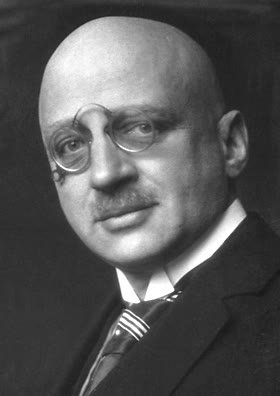
\includegraphics[width=\linewidth]{images/book2/haber.jpg}
\end{minipage}\hfill
\begin{minipage}[t]{0.78\linewidth}\vspace{0pt}
Fritz Haber showed that ammonia could be made from nitrogen and hydrogen
under pressure over a \omterm{def:b1:elementary-steps:catalyst}{catalyst}; Carl Bosch turned the laboratory reaction
into an industrial process. Haber received the Nobel Prize in Chemistry
for 1918. The same man directed the first large-scale use of chlorine as
a weapon in the First World War: chemistry that feeds half of humanity
and chemistry that kills are separated by the choices of chemists.
(Photograph: The Nobel Foundation, published 1919, public domain,
Wikimedia Commons.)
\end{minipage}
\end{history}

\section{Phosphorus and the trends down the groups}

Phosphorus, below nitrogen, does not form \ce{P#P} triple bonds: white
phosphorus is made of \ce{P4} tetrahedra, strained and reactive (it
ignites in air and is kept under water); red phosphorus is a polymer,
much less reactive. Burning phosphorus gives \ce{P4O10}, the most acidic
of the common oxides, which with water gives phosphoric acid,
$\mathrm{p}K_a$ 2.15, 7.21, 12.34 (\cref{ch:b1:predominant-reaction}).
Phosphate rock, mined at about 250 million tonnes in 2025, is turned by
sulfuric acid into phosphate fertilisers.
% ledger: usgs:phosphate-world-2025

Down each group the elements become more metallic (boron to thallium,
carbon to lead, nitrogen to bismuth), their oxides more basic, and the
lower oxidation states more stable: the \omterm{def:b1:p-block-13-15:inert-pair}{inert-pair effect}. Across a
\omterm{def:b1:periodicity:table}{period}, the oxides become more acidic, from basic \ce{Na2O} to the \omterm{def:b1:s-block:oxide-character}{acidic
oxides} of phosphorus and sulfur.

\section{Exercises}

\begin{exercise}[$\star$]\label{exo:b1:p-block-13-15:1}
Give the \omterm{def:b1:nernst:oxidation-number}{oxidation number} of nitrogen in \ce{NH4NO3} (both atoms),
\ce{N2O5}, \ce{HNO2}, \ce{N2H4} and \ce{Mg3N2}.
\end{exercise}

\begin{exercise}[$\star$]\label{exo:b1:p-block-13-15:2}
Draw the \omterm{def:b1:lewis-resonance-vsepr:lewis}{Lewis structures} of \ce{BF3}, \ce{NH3} and of the adduct
\ce{F3B-NH3}; identify the \omterm{def:b1:lewis-resonance-vsepr:lewis-acid}{Lewis acid} and base.
\end{exercise}

\begin{exercise}[$\star$]\label{exo:b1:p-block-13-15:3}
Write the reactions of \ce{CO2}, \ce{SiO2} (molten) and \ce{P4O10} with
sodium hydroxide, and of \ce{Al2O3} with an acid and a base.
\end{exercise}

\begin{exercise}[$\star$]\label{exo:b1:p-block-13-15:4}
Compute the equilibrium constant of \ce{N2 + 3H2 <=> 2NH3} at
\qty{25}{\celsius} from $\Delta_f G^\circ(\ce{NH3}) =
\qty{-16.45}{kJ/mol}$.
\end{exercise}

\begin{exercise}[$\star\star$]\label{exo:b1:p-block-13-15:5}
Using the counting of \cref{prop:b1:p-block-13-15:silicate-units}, give the
formula of a ring of six tetrahedra each sharing two corners (as in beryl)
and of a double chain in which half the tetrahedra share two corners and
half share three.
\end{exercise}

\begin{exercise}[$\star\star$]\label{exo:b1:p-block-13-15:6}
Compute the mass of alumina obtained from one tonne of bauxite containing
\qty{55}{\percent} of \ce{Al(OH)3} by mass, with \qty{92}{\percent}
recovery.
\end{exercise}

\begin{exercise}[$\star\star$]\label{exo:b1:p-block-13-15:7}
Show that boric acid is a \omterm{def:b1:lewis-resonance-vsepr:lewis-acid}{Lewis acid} rather than a \omterm{def:b1:predominant-reaction:bronsted}{Brønsted acid}, and
explain why its solution is nevertheless acidic.
\end{exercise}

\begin{exercise}[$\star\star$]\label{exo:b1:p-block-13-15:8}
Balance the oxidation of ammonia to \ce{NO} with the \omterm{def:b1:nernst:oxidation-number}{oxidation numbers} and
give the number of electrons exchanged per \ce{NH3}.
\end{exercise}

\begin{exercise}[$\star\star$]\label{exo:b1:p-block-13-15:9}
Ammonium nitrate is made from ammonia and nitric acid. Write the reaction,
and compute the mass of ammonia needed (both for the nitric acid and for
the neutralisation) per tonne of ammonium nitrate.
\end{exercise}

\begin{exercise}[$\star\star\star$]\label{exo:b1:p-block-13-15:10}
Explain why nitrogen is a diatomic gas and phosphorus a solid of \ce{P4}
molecules, and why carbon dioxide is a gas and silica a solid, using the
strength of $\pi$ bonds between \omterm{def:b1:periodicity:table}{second-period} and \omterm{def:b1:periodicity:table}{third-period} atoms.
\end{exercise}

\begin{exercise}[$\star\star\star$]\label{exo:b1:p-block-13-15:11}
Show with the \omterm{def:b1:nernst:electrode-potential}{standard potentials} that lead(IV) oxide oxidises chloride
ions to chlorine in acid, whereas silicon(IV) oxide does nothing of the
sort. Relate this to the \omterm{def:b1:p-block-13-15:inert-pair}{inert-pair effect}.
\end{exercise}

\begin{exercise}[$\star\star\star$]\label{exo:b1:p-block-13-15:12}
The world produced about 160 million tonnes of nitrogen as ammonia in 2025.
What mass of ammonia is that, and what mass of hydrogen did it contain?
Where does that hydrogen mostly come from?
\end{exercise}

\section{Problem: From Air to Fertiliser}

\begin{problem}[{Weekend problem --- the nitrogen triple bond, ammonia
synthesis, the three steps of nitric acid manufacture, ammonium nitrate,
and the mass of nitric acid obtainable from one tonne of ammonia}]
\label{pb:b1:p-block-13-15:1}
A fertiliser plant converts ammonia into nitric acid and ammonium
nitrate. Molar masses (\unit{g/mol}): \ce{N2} 28.0, \ce{H2} 2.0, \ce{NH3}
17.0, \ce{HNO3} 63.0, \ce{NH4NO3} 80.0, \ce{O2} 32.0;
$\Delta_f G^\circ(\ce{NH3(g)}) = \qty{-16.45}{kJ/mol}$ at
\qty{25}{\celsius}.

\medskip
\noindent\textbf{Part I --- Nitrogen.}
\begin{enumerate}
  \item Draw the \omterm{def:b1:lewis-resonance-vsepr:lewis}{Lewis structure} of \ce{N2} and say why it is unreactive.
  \item Give the \omterm{def:b1:nernst:oxidation-number}{oxidation number} of N in \ce{N2}, \ce{NH3}, \ce{NO},
        \ce{NO2}, \ce{HNO3} and \ce{NH4NO3}.
  \item Name three natural or industrial ways of fixing nitrogen.
  \item Why are plants unable to use \ce{N2} directly?
  \item Which element is oxidised and which reduced in the synthesis of
        ammonia?
  \item Write the synthesis of ammonia.
\end{enumerate}

\medskip
\noindent\textbf{Part II --- Ammonia.}
\begin{enumerate}[resume]
  \item Compute the equilibrium constant of the synthesis at
        \qty{25}{\celsius}.
  \item Why is the synthesis nevertheless run hot, over a \omterm{def:b1:elementary-steps:catalyst}{catalyst}?
  \item Compute the masses of \ce{N2} and \ce{H2} for one tonne of
        ammonia.
  \item What volume of air (\qty{78}{\percent} \ce{N2} by volume, ideal
        gas, \qty{25}{\celsius}, \qty{1}{bar}) contains that nitrogen?
  \item Where does the hydrogen come from?
  \item Why is ammonia itself used as a fertiliser in some countries, and
        why is it often converted first?
\end{enumerate}

\medskip
\noindent\textbf{Part III --- Nitric acid.}
\begin{enumerate}[resume]
  \item Balance step 1, \ce{NH3 + O2 -> NO + H2O}, with \omterm{def:b1:nernst:oxidation-number}{oxidation numbers}. % ce-unbalanced-ok
  \item Balance step 2, \ce{NO + O2 -> NO2}. % ce-unbalanced-ok
  \item Balance step 3, \ce{NO2 + H2O -> HNO3 + NO}. Which kind of redox % ce-unbalanced-ok
        reaction is it?
  \item Combine the steps with complete recycling of NO into the overall
        equation.
  \item Compute the mass of oxygen consumed per tonne of ammonia.
  \item Why is a platinum--rhodium gauze used in step 1?
\end{enumerate}

\medskip
\noindent\textbf{Part IV --- Ammonium nitrate and mass balances.}
\begin{enumerate}[resume]
  \item Write the formation of ammonium nitrate.
  \item What fraction of the ammonia must be turned into nitric acid to
        make only ammonium nitrate?
  \item Compute the mass of ammonium nitrate from one tonne of ammonia
        shared in that way.
  \item What percentage of nitrogen does ammonium nitrate contain?
  \item Why must ammonium nitrate be stored away from fuels and heat?
  \item Compute the mass of nitric acid obtainable from one tonne of
        ammonia (complete conversion).
\end{enumerate}
\end{problem}
